\documentclass{standalone}
\usepackage{tikz}
\usetikzlibrary{decorations.pathmorphing,patterns}
\begin{document}
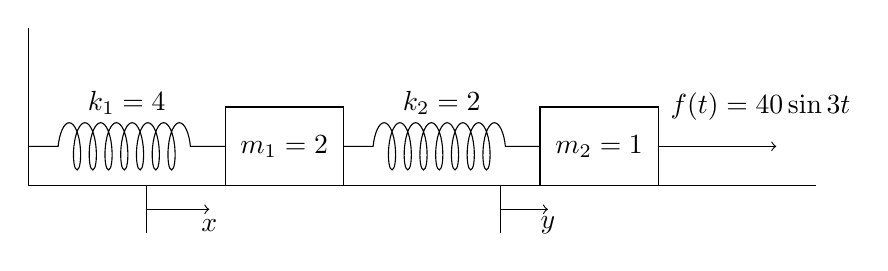
\begin{tikzpicture}
\draw (-2,0) -- (8,0);
\draw (-2,0) -- (-2,2);
\draw (-0.5,0) -- (-0.5,-0.6);
\draw [->] (-0.5,-0.3) -- (0.3,-0.3);
\draw (0.3,-0.5) node {$x$};
\draw (4,0) -- (4,-0.6);
\draw [->] (4,-0.3) -- (4.6,-0.3);
\draw (4.6,-0.5) node {$y$};
\draw[decoration={aspect=0.3, pre length = 3.8mm, post length =3mm, segment length=2mm, amplitude=3mm,coil},decorate] (-2,0.5) -- (0.5,0.5) node [midway, above = 8] {$k_{1}=4$}; 
\draw (0.5,0) rectangle (2, 1) node [pos=0.5] {$m_{1}=2$};
\draw[decoration={aspect=0.3, pre length = 3.8mm, post length =3mm, segment length=2mm, amplitude=3mm,coil},decorate] (2,0.5) -- (4.5,0.5) node [midway, above = 8] {$k_{2}=2$}; 
\draw (4.5,0) rectangle (6, 1) node [pos=0.5] {$m_{2}=1$};
\draw (7.3, 1) node {$f(t) = 40 \sin 3t$};
\draw [->] (6,0.5) -- (7.5,0.5);
\end{tikzpicture}
\end{document}